% abstract_takada.tex
% #################################################

\documentclass{article_vdlab_sotsuron_youshi}
\pagestyle{empty}

\usepackage{setspace}
\usepackage{graphicx}
\usepackage{amsmath,amssymb}
\usepackage{comment}
\usepackage{here}

%2段組みの段組み間間隔を設定
\columnsep=1.5cm

\begin{document}
%文字間隔の設定
\kanjiskip = .7pt plus3pt minus 3pt
\xkanjiskip = .7pt plus 3pt minus 3pt
\small
\setstretch{1.1}

%図回りの余白を設定
\setlength{\abovecaptionskip}{0mm}
\setlength{\belowcaptionskip}{0mm}
\setlength{\floatsep}{0mm}
\setlength{\textfloatsep}{0mm}
\setlength{\intextsep}{3mm}
\setlength{\dblfloatsep}{0mm}
\setlength{\dbltextfloatsep}{0mm}

% #################################################

\twocolumn[
  \begin{center}
    % 論文題目と氏名
    \jtitle{タイヤ-サスペンションHILSシステムにおける上下動再現手法の検討}
    \jauthors{高田 茉莉乃}
    \etitle{Study on Reproduction Method of Vertical Motion with Tire-Suspension\\Hardware-in-the-Loop Simulation System}
    \eauthors{Marino TAKADA}
  \end{center}
]

%文字間隔の設定
\kanjiskip = .7pt plus3pt minus 3pt
\xkanjiskip = .7pt plus 3pt minus 3pt
\small
\setstretch{1.1}

% #################################################
\section{緒言}
HILSシステムとは,Hardware-in-the-Loop Simulationの略称であり,対象のハードウェアをシミュレーションループ内に直接組み込むことで特性評価を行うシステムである.タイヤ-サスペンション系に含まれるダンパは非線形特性を有するため,シミュレーションによる評価は難しい.一方,実車走行試験による評価では,路面状況や天候などの影響により測定値のばらつきが大きいことや同一条件で試験を行うことが困難である.このような問題を解決するシステムとしてHILSシステムが用いられている\cite{2}.\par
本研究では,自動車のタイヤ-サスペンション系の上下動をHILSシステムを用いて評価する.タイヤ-サスペンション系をHILSシステムに組み込む場合,ハードウェア部の構成は,車体部を固定し,路面部のアクチュエータを制御する1自由度系と,車体部を固定せず,路面と車体の変位をそれぞれ制御する2自由度系が考えられる.ハードウェア部の構成がHILSの再現性に与える影響を評価するため,1自由度系と2自由度系の両方の構成が可能な試験装置を新たに開発し,HILSシステムを構築した.両システムにおいて試験装置と解析モデルの差を比較することにより,上下動の再現性を評価した.

% #################################################
\section{タイヤ-サスペンションHILSシステム}
\vspace*{-1mm}
\subsection{HILSシステムの構成}
本研究で新たに構築したHILSシステムの概要を図~\ref{fig:HILS}~に示す.このHILSシステムは,車両運動解析やシステム制御を行うソフトウェア部と,ハードウェア部である試験装置から構成される.本システムでは試験装置のばね上-ばね下相対変位が解析結果と一致するように制御を行う.解析モデルには上下2自由度モデルを用いる.試験装置から計測されたダンパ力を用いてリアルタイム車両運動解析を実行し,ばね上-ばね下間相対変位を算出する.この解析結果に基づいてモータを制御することで,車両の上下動を再現する.

\begin{figure}[H]
  \begin{center}
    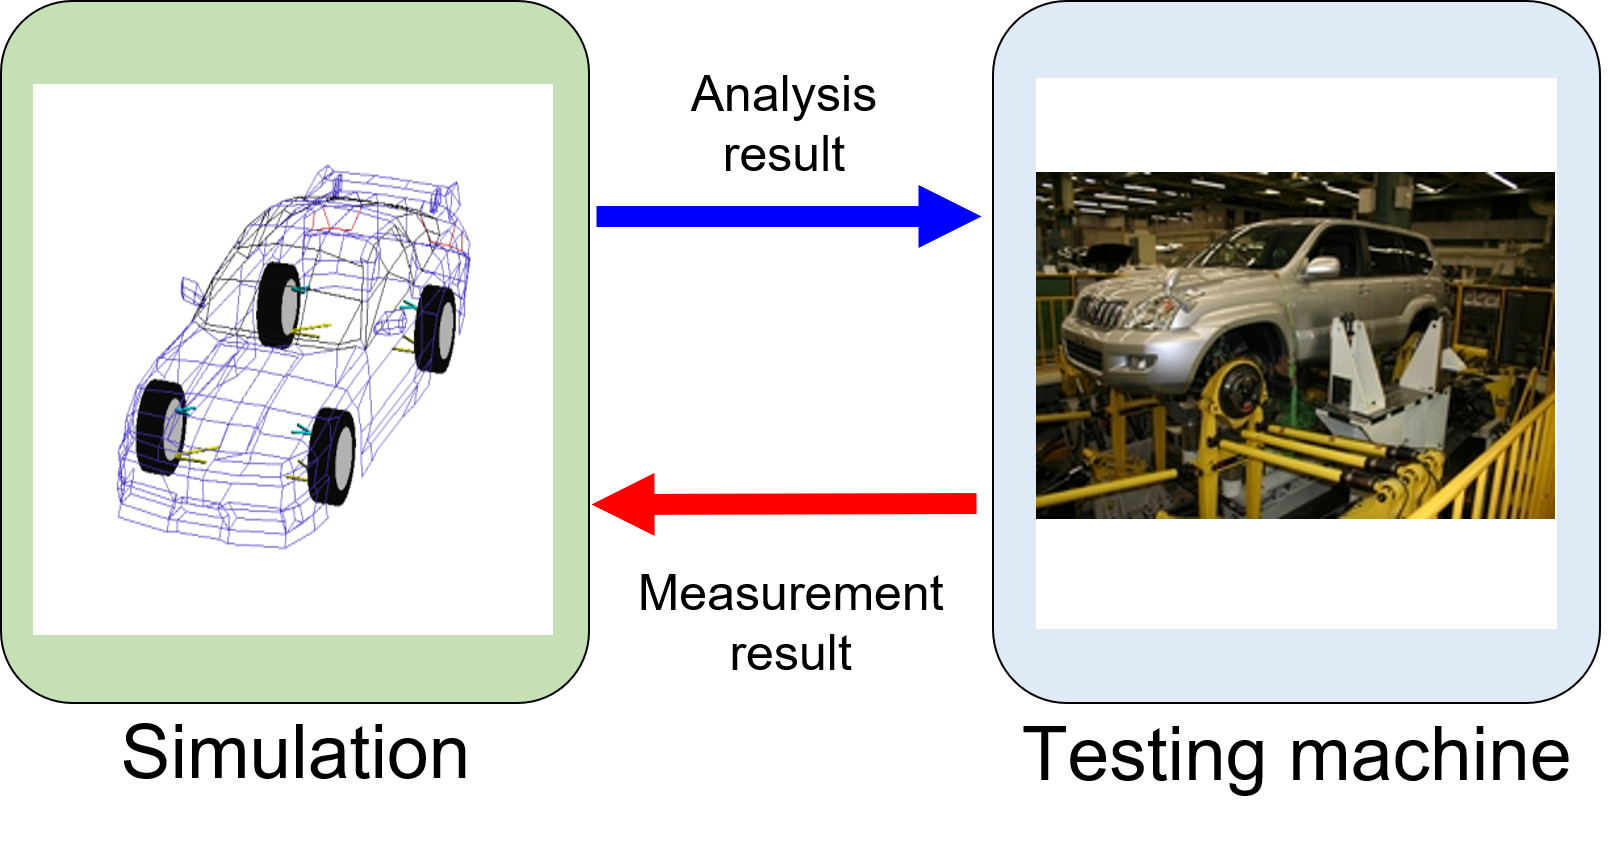
\includegraphics[height=70mm]{figure/HILS.eps}
    \vspace*{-2mm}
    \caption{System Overview of Tire-Suspension HILS System}
    \label{fig:HILS}
  \end{center}
\end{figure}

\vspace*{-5mm}
解析モデルに用いた上下2自由度モデルは,車両の上下動を表すことのできるモデルである\cite{7}.上下2自由度モデルを図~\ref{fig:analysis_model}~に示す.また,このモデルの運動方程式は以下である.

\vspace*{-5mm}
\begin{flalign}
 \label{eq:1} &m_1\ddot x_1 + k_1(x_1-x_0) + k_2(x_1-x_2) - f_c = 0\\
 \label{eq:2} &m_2\ddot x_2 + k_2(x_2-x_1) + f_c = 0
\end{flalign}

\noindent
ここで,$m_1$はばね下質量 ,$m_2$はばね上質量,$k_1$,$k_2$はばね定数,$f_c$はダンパ力,$x_0$は路面変位,$x_1$はばね下変位,$x_2$はばね上変位である.

\begin{figure}[H]
    \begin{center}
      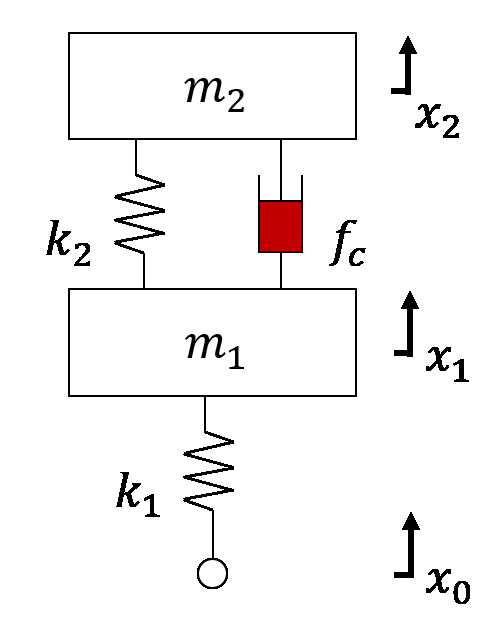
\includegraphics[height=30mm]{figure/analysis_model.eps}
      \vspace*{1mm}
      \caption{Analysis Model}
      \label{fig:analysis_model}
    \end{center}
\end{figure}

% **************************************************
\vspace*{-5mm}
\subsection{システム構成の違い}
1自由度系HILSシステムと2自由度系HILSシステムのハードウェアの概略図を図~\ref{fig:1dof_2dof}~に示す.図~\ref{fig:1dof_2dof}~(a) の1自由度系HILSシステムのアクチュエータAには,解析モデルから算出されたばね上-ばね下相対変位に基づき,路面入力を決定する.アクチュエータが1つであるためハードウェア構成が単純になるが,アクチュエータは装置の荷重を支えつつ高い応答性を要求される.図~\ref{fig:1dof_2dof}~(b) の2自由度系HILSシステムは,ばね上変位と路面変位をそれぞれ別のアクチュエータによって制御する.アクチュエータAには解析モデルと同じ路面入力を与え,アクチュエータBは解析結果に基づいたばね上変位を制御する.ハードウェアへの入力が2つとなり構成が複雑になるが,装置の荷重をアクチュエータAが支えるため,解析結果に基づいて制御を行うアクチュエータBにかかる負荷が軽減できる.

\vspace*{-2mm}
\begin{figure}[H]
  \begin{tabular}{cc}
  \begin{minipage}{0.5\hsize}
    \vspace*{6mm}
  \begin{center} 
    \hspace*{8mm}
    \includegraphics[height=35mm]{figure/1dof_model.eps}
    \end{center}
    \begin{center}
    \vspace*{-4mm}
    \ (a) 1DOF HILS\
%     \label{fig:1dof_model} 
    \end{center}
  \end{minipage}
  \hspace*{-5mm}
  \begin{minipage}{0.4\hsize}
     \begin{center}
     \hspace*{8mm}
      \includegraphics[height=40mm]{figure/2dof_model.eps}
      \end{center}
      \begin{center}
      \vspace*{-4mm}
      \ (b) 2DOF HILS\
%       \label{fig:2dof_model}
    \end{center}
  \end{minipage}
  \end{tabular}
    \vspace*{1mm}
    \caption{Hardware of HILS System}
    \label{fig:1dof_2dof}
 \end{figure}

% #################################################
\section{試験装置の開発}
\vspace*{-1mm}
\subsection{試験装置の概要}
開発した試験装置を図~\ref{fig:testing_machine}~に,諸元を表~\ref{tab:parameter}~に示す.本試験装置は解析モデルと同じ上下2自由度系を模擬してあり,可動部は路面部,タイヤに相当するばね下,車体に相当するばね上から構成される.ばね上を外枠フレームに対して固定し,アクチュエータBを取り外すことで1自由度系を再現できる.上下に可動する部分にはリニアベアリングを取り付けた.路面部はスライダ-クランク機構を,車体部はボールねじ機構を介してアクチュエータにより位置決め制御される.アクチュエータAにはギア比が高く,トルクを重視したモータを,アクチュエータBにはギア比が低く,応答性を重視したモータを選定した.ダンパ力は1軸ロードセル,ばね下変位はレーザ変位計を用いて計測する.

\begin{figure}[H]
  \begin{minipage}{0.6\hsize}
    \begin{center}
      \includegraphics[height=50mm]{figure/testing_machine.eps}
      \vspace*{-1mm}
      \caption{Testing Machine}
    \label{fig:testing_machine}
    \end{center}
  \end{minipage}
  \begin{minipage}{0.35\hsize}
      \begin{center}
	\makeatletter
	\def\@captype{table}   
	\makeatother
	\caption{Parameter}
	\label{tab:parameter}
	  \begin{tabular}{cc}\hline
	    $m_1$ [kg] & 1.5\\
	    $m_2$ [kg] & 6.4\\
	    $k_1$ [N/m] & 2200\\
	    $k_2$ [N/m] & 405\\
	    $c_2$ [N/m] & 7\\\hline 
	  \end{tabular}  
      \end{center}
  \end{minipage}
\end{figure}

% **************************************************
\vspace*{-1mm}
\subsection{モータ単体の応答特性}
モータの応答特性を検証するため,スイープ波入力試験を実施した.路面部のモータは加速度一定,ばね上のモータはボールねじの変位限界があることから,変位一定のスイープ波を入力した.それぞれのボード線図を図~\ref{fig:sweep}~に示す.入力はモータの回転角,出力はエンコーダから計測した回転角である.両者ともにゲインがフラットな特性を示したので,モータの周波数応答性は良いと言える.

\vspace*{-2mm}
\begin{figure}[H]
  \begin{tabular}{cc}
  \begin{minipage}{0.5\hsize}
  \begin{center} 
    \includegraphics[clip,width=45mm]{figure/ecmax40_sweep.eps}
  \end{center}
  \vspace*{-13mm}
  \begin{center}
    \ (a) Actuator A\
%     \label{fig:ecmax40_sweep}
  \end{center}
  \end{minipage}
  \hspace*{-4mm}
  \begin{minipage}{0.45\hsize}
    \begin{center}
      \includegraphics[clip,width=45mm]{figure/ec22_sweep.eps}
    \end{center}
    \vspace*{-13mm}
    \begin{center}
      \ (b) Actuator B\
%       \label{fig:ec22_sweep}
    \end{center}
  \end{minipage}
  \end{tabular}
    \vspace*{1mm}
    \caption{Boad Diagram}
    \label{fig:sweep}
\end{figure}

% #################################################
\vspace*{-2mm}
\section{HILSにおける上下動再現手法の検討}
\subsection{1自由度系HILSシステムと2自由度系HILSシステムの比較}
1自由度系HILSシステムと2自由度系HILSシステムにおける上下動の再現性を評価するために,路面入力試験を行った.図~\ref{fig:compare_2_7}~に周波数2.0Hz,振幅7mmの正弦波を,図~\ref{fig:compare_5_2}~に周波数5Hz,振幅2mmの正弦波を路面に入力した際の,サスペンションストロークを比較したグラフを示す.\par
図~\ref{fig:compare_2_7}~のように入力周波数が低い場合は,解析結果とハードウェアの計測値が同じ挙動を示したため,上下動の再現性は高いと言える.しかし,図~\ref{fig:compare_2_7}~(a) の1自由度系HILSシステムでは,解析結果に対して計測値が僅かに遅れていることがわかる.これは,解析モデルとハードウェアの動特性が異なるためであると考えられる.また,図~\ref{fig:compare_5_2}~のように入力周波数が高くなると,特に1自由度系HILSシステムで解析結果と計測値の振幅が離れた.これは,解析モデルとハードウェアの動特性が異なるためであると考えられる.

\vspace*{2mm}
\hspace*{5mm}
\begin{tabular}{cc}
  \begin{minipage}{0.7\hsize}
    \begin{center} 
      \includegraphics[height=33mm]{figure/1_sine_2_7.eps}
%       \includegraphics[height=33mm]{figure/1_sine_2_7_gray.eps}
      \end{center}
      \begin{center}
      \vspace*{-4mm}
      \ (a) 1DOF HILS\
%       \label{fig:1_sine_2_7} 
    \end{center}
  \end{minipage}
  \hspace*{-12mm}
  \begin{minipage}{0.3\hsize}
    \includegraphics[height=10mm]{figure/legend.eps}
%     \includegraphics[height=10mm]{figure/legend_gray.eps}
  \end{minipage}
\end{tabular}

\vspace*{-3mm}
\begin{figure}[H]
  \hspace*{9mm}
  \begin{tabular}{cc}
  \begin{minipage}{0.7\hsize}
    \begin{center} 
      \includegraphics[height=33mm]{figure/2_sine_2_7.eps}
%       \includegraphics[height=33mm]{figure/2_sine_2_7_gray.eps}
      \end{center}
      \begin{center}
      \vspace*{-6mm}
      \ (b) 2DOF HILS\
%       \label{fig:1_sine_2_7} 
    \end{center}
  \end{minipage}
  \begin{minipage}{0.3\hsize}
    \hspace*{-12mm}
    \includegraphics[height=10mm]{figure/legend.eps}
%     \includegraphics[height=10mm]{figure/legend_gray.eps}
  \end{minipage}
  \end{tabular}
  \vspace*{1mm}
  \caption{Comparision of HILS (Input: 2Hz,7mm)}
  \label{fig:compare_2_7}
\end{figure}

% 隠れ全角スペース
 

\hspace*{5mm}
\begin{tabular}{cc}
  \begin{minipage}{0.7\hsize}
    \begin{center} 
      \includegraphics[height=33mm]{figure/1_sine_5_2.eps}
%       \includegraphics[height=33mm]{figure/1_sine_5_2_gray.eps}
      \end{center}
      \begin{center}
      \vspace*{-4mm}
      \ (a) 1DOF HILS\
%       \label{fig:1_sine_5_2} 
    \end{center}
  \end{minipage}
  \begin{minipage}{0.3\hsize}
    \hspace*{-12mm}
    \includegraphics[height=10mm]{figure/legend.eps}
%     \includegraphics[height=10mm]{figure/legend_gray.eps}
  \end{minipage}
\end{tabular}

\vspace*{-3mm}
\begin{figure}[H]
  \hspace*{9mm}
  \begin{tabular}{cc}
  \begin{minipage}{0.7\hsize}
    \begin{center} 
      \includegraphics[height=33mm]{figure/2_sine_5_2.eps}
%       \includegraphics[height=33mm]{figure/2_sine_5_2_gray.eps}
      \end{center}
      \begin{center}
      \vspace*{-6mm}
      \ (b) 2DOF HILS\
%       \label{fig:1_sine_5_2} 
    \end{center}
  \end{minipage}
  \begin{minipage}{0.3\hsize}
    \hspace*{-12mm}
    \includegraphics[height=10mm]{figure/legend.eps}
%     \includegraphics[height=10mm]{figure/legend_gray.eps}
  \end{minipage}
  \end{tabular}
  \vspace*{1mm}
  \caption{Comparision of HILS (Input: 5Hz,2mm)}
  \label{fig:compare_5_2}
\end{figure}

% #################################################
 \vspace*{-2mm}
\section{結言}
本研究では,タイヤ-サスペンション系の上下動を,HILSシステムを用いて評価した.1自由度系と2自由度系の両方のハードウェア構成が可能な試験装置を開発し,HILSシステムを構築した.正弦波入力試験を実施し,1自由度系HILSシステムと2自由度系HILSシステムの上下動の再現性を比較した.周波数が低い領域では両者とも再現性が高いが,高周波領域になると上下動の再現性が低下することがわかった.よって,2自由度系HILSシステムのほうが上下動の再現性が高いと言える.

\begin{thebibliography}{9}
  \bibitem{2}永井正夫,吉田秀久,Noomwongs Nuksit,横井隆,川眞田智,小林克宏,タイヤHIL シミュレータによる車両運動性能の研究(第1 報) : タイヤHIL シミュレータの開発,自動車技術会論文集,Vol35,No. 2,(2004),pp. 147-152
  \bibitem{7}社団法人\ 自動車技術会,自動車技術ハンドブック5設計(シャシ)編,社団法人\ 自動車技術会,(1990),p. 25
\end{thebibliography}

\end{document}
